\begin{table}[!ht]
    % 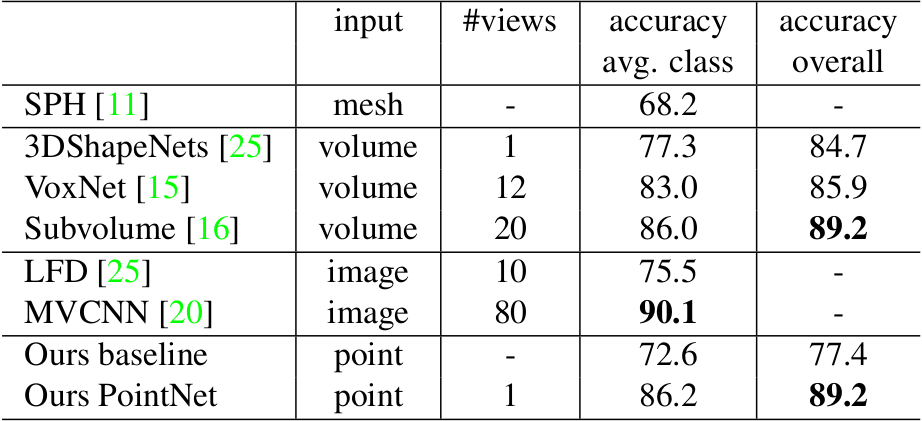
\includegraphics[width=0.5\textwidth]{modelnet}
    \normalsize
    \begin{tabular}{l|c|c|c|c}
        & input & \#views & accuracy & accuracy \\
        & & & avg. class & overall \\ \hline
        SPH \cite{kazhdan2003rotation} & mesh & - & 68.2 & - \\ \hline

        3DShapeNets \cite{wu20153d}     & volume & 1 & 77.3 & 84.7 \\
        VoxNet \cite{maturana2015voxnet} & volume & 12 & 83.0 & 85.9 \\
        Subvolume \cite{qi2016volumetric} & volume & 20 & 86.0 & \textbf{89.2} \\ \hline

        LFD \cite{wu20153d} & image & 10 & 75.5 & - \\
        MVCNN \cite{su2015multi} & image & 80 & \textbf{90.1} & - \\ \hline

        Ours baseline & point & - & 72.6 & 77.4 \\
        Ours PointNet & point & 1 & 86.2 & \textbf{89.2} \\
    \end{tabular}
    \caption{
        \textbf{Classification results on ModelNet40.}
        PointNet achieves state-of-the-art among deep nets on 3D input.
        % Our net achieves
        % state-of-the-art among deep nets on 3D input." Table and caption taken
        % from \cite{qi2017pointnet}. \todo{rewrite in own words}
        Table from \cite{qi2017pointnet}.
    } \label{table:modelnet}
\end{table}
